

%(BEGIN_QUESTION)
% Copyright 2012, Tony R. Kuphaldt, released under the Creative Commons Attribution License (v 1.0)
% This means you may do almost anything with this work of mine, so long as you give me proper credit

En SMART DP-celle er tatt ut av drift og tatt med for benkkalibrering. En automatikker kobler til et presisjons trykkmanometer og en luftkilde til High inngangen på DP-cellen, mens han måler strømutgangen med et multimeter. 

$$\includegraphics[width=15.5cm]{if002x01.eps}$$

Regn ut avviket i \% av måleområde for {\it sensor trim} og avviket i  \% av måleområde for {\it utgangstrim}.  Forklar hvorfor en må ha en HART kommunikator for å kunne regne disse avvikene sepparat. 
\eject

\begin{tikzpicture}
	\draw[step=0.5cm,gray!20,very thin]  grid (16,16) ;
\end{tikzpicture}
%\vskip 20pt \vbox{\hrule \hbox{\strut \vrule{} {\bf Suggestions for Socratic discussion} \vrule} \hrule}

%\begin{itemize}
%\item{} What other possible sources of error besides the transmitter could account for these discrepancies?
%\item{} Suppose another instrument technician suggests to you that a problem within the precision air pressure regulator might account for some (or all!) of the calibration error seen in the data, and that we should replace the regulator with another.  How would you respond to this suggestion?
%\item{} Suppose another instrument technician suggests to you that a problem within the loop resistor might account for some (or all!) of the calibration error seen in the data, and that we should replace the resistor with another.  How would you respond to this suggestion?
%\item{} Does the HART communicator need to be NIST traceable?  Why or why not?
%\end{itemize}

\underbar{file if002.tex}
%\underbar{file i02033}
%(END_QUESTION)





%(BEGIN_ANSWER)


%(END_ANSWER)





%(BEGIN_NOTES)

$$\hbox{Sensor trim error:} \hskip 20pt \left({28.75 - 28.70 \over 35}\right) 100\% = +0.142857\%$$

$$\hbox{Output trim error:} \hskip 20pt \left({17.53 - 17.14 \over 16}\right) 100\% = +2.4375\%$$


%INDEX% Calibration, smart transmitter: digital trim
%INDEX% Fieldbus, HART: communicator variables
%INDEX% Measurement, pressure: troubleshooting

%(END_NOTES)

